\documentclass[11pt,a4paper]{report}	% report - article
\usepackage{graphicx}
\usepackage{fancyhdr} 
\usepackage{fancybox} 
\usepackage{psfrag}
\usepackage{boxedminipage} 
\usepackage{epsfig}
\usepackage{amsmath}
\usepackage[ngerman]{babel}
\usepackage[T1]{fontenc}	%fr Sonderzeichen s. latin1
\usepackage[latin1]{inputenc}   %fr Umlaute & scharfes s
\usepackage{times}
\usepackage{float}
\usepackage{amsmath,amssymb}
\usepackage[dvips, a4paper, raiselinks, breaklinks, colorlinks, bookmarks, bookmarksnumbered,citecolor = black, linkcolor = black]{hyperref}
\usepackage{zardozDipl} 
\usepackage{url}







%
%
%\fancypagestyle{plain}{%
%    \lhead{LaTeX - TeXnicCenter} %left head
%    \rhead{Vorlage V2.0} % right head
%    \lfoot{Institut fr Robotik}
%    \rfoot{\thepage}
%    \cfoot{}		%keine Seitenangabe zustzlich in der Mitte !!!
%    \renewcommand{\headrulewidth}{0.4pt}
%    \renewcommand{\footrulewidth}{0.4pt}
%}
%
\pagestyle{plain}
%
\pagenumbering{arabic}
%
%\newtheorem{Aufgabe}{Aufgabe}[section]
%\newtheorem{Hinweis}{Hinweis}[section]
%
%
%\renewcommand{\chaptermark}[1]{}%   %shows chapter left header
%     
\renewcommand{\sectionmark}[1]{\markright{\thesection\ #1}{}}
%
\newcommand{\qu}{\symbol{94}}  %"^" !!!
\newcommand{\MS}{MatLab/SimuLink }
%
%--------------------------------------------------
%
\setlength{\parindent}{0mm}




\setcounter{section}{0}

\begin{document}

		%\textwidth 16cm
%\textheight 25cm
%\topmargin 3.2cm
%\oddsidemargin 0mm
%\parindent 0pt

\thispagestyle{empty}

% Verschiebung der Coverpage in X und Y. Einheit in cm.
\def\DELTAX{0.8}
\def\DELTAY{4.0}


% -------- only change entries beginning here ----------------------------
%
% enter the title of the thesis
%
\def\title{Leonardo da Vinci Program }
%
% choose type of work: 0 ... Dissertation
%                      1 ... Diplomarbeit
%                      2 ... Masterarbeit
\def\type{1}
%
%
% enter name of degree, see examples below
%
\def\degree{Internship}
%\def\degree{Diplomingenieurin}
%\def\degree{Master of Science}
%\def\degree{Doktor}
%\def\degree{Doktorin}

% enter the study (Studienrichtung)
% e.g. Diplomstudium:
%\def\study{Technische Mathematik}
% e.g. Masterstudium:
% \def\study{Industriemathematik}
% e.g. Doktorratsstudium
%\def\study{Technischen Wissenschaften}
%\def\study{Naturwissenschaften}
\def\study{Mechatronik}


% enter the name of the student
%
\def\name{Aaron Martinez Romero}
%
%
% enter the name of the institute
% e.g.
% \def\institute{Institut f\"ur Industriemathematik}
%
\def\institute{Institut f\"ur Robotik}
%
%
% enter the name of the supervisor (who is also the first referee)
% was also the supervisor, do so by choosing the line with (Betreuung)
%
\def\firstreferee{o. Univ.--Prof.\ Dr.--Ing.\ habil.\ Hartmut\ Bremer}
%
%
% in case of a second referee: uncomment the following line and enter the name
%
%\def\secondreferee{Prof.\ Dr.--Ing.\ habil.\ Dr. h.c. i.R.\ Max \ Muster}
%
%
% if there has been assistance by further people uncomment the following line
% and enter the name(s). if there are several assistants speerate the names by \\
%
 \def\assist{Name of assistant}
%\def\assist{Name of first assistant \\ Name of second assistant}
%
%
% enter month year
\def\date{March, 2011}
%
%
% the vertival alignment heavily depends on the length of the title if there are
% one or two supervisors or referees. whereever indicated as a question
%      more space ???
% below you might add additional space via (several) \medskip or \bigskip.
% do not change anything else
% -------------------------------------------------------------------------------
%
\def\ifundefined#1{\expandafter\ifx\csname#1\endcsname\relax}
%
\unitlength 1cm



\sffamily
\begin{picture}(0,0)(\DELTAX,\DELTAY)
\put(-2.6,5){\color{blue}\rule{25cm}{2.6cm}}
\put(10.8,5.15){\small UNIVERSIT\"AT}
\put(13.62,5.15){\small LINZ}
\put(10.8,5.5){\small JOHANNES}
\put(13,5.5){\small KEPLER}
\put(15,5.15){\Huge JKU}
\put(14.75,5.15){\line(0,1){.6}}
%\put(9.7,5.6){
\includegraphics[width=9mm]{img/wap_small.png}}
%\put(0,1){
\includegraphics[width=3cm]{img/tnf.png}}
\put(3.2,1.4){\scriptsize Technisch-Naturwissenschaftliche}
\put(3.2,1.05){\scriptsize Fakult\"at}
\end{picture}
%
\vspace{\DELTAY cm}

\begin{center}
{\LARGE\bfseries\title}
\bigskip\bigskip\bigskip\par
{\Large\ifcase\type DISSERTATION\or DIPLOMARBEIT\or MASTERARBEIT\fi}
\bigskip\par
zur Erlangung des akademischen Grades
\bigskip\smallskip\par
{\Large\degree}
\bigskip\par
im \ifcase\type Doktoratsstudium der\or Diplomstudium\or Masterstudium\fi
\bigskip\smallskip\par
{\Large\study}
\end{center}
%
% more space ???
%\bigskip
\bigskip\bigskip\bigskip\par
Eingereicht von:
\smallskip\par
{\large\name}
\medskip\bigskip\par
Angefertigt am:
\smallskip\par
{\large\institute}
\medskip\bigskip\par
Beurteilung:
\smallskip\par
{\large\firstreferee}
\ifundefined{secondreferee}\else {\large (Betreuung)}
\smallskip\par
{\large\secondreferee}\fi
\ifundefined{assist}\else
\medskip\bigskip\par
Mitwirkung:
\smallskip\par
{\large\assist}
\fi
%
% more space ???
%\bigskip
\bigskip\bigskip\bigskip\par
{\large Linz, \date}

\rmfamily 
	

		\pagestyle{zardoz}
		
		\textheight 24cm
		\textwidth 16cm
		\oddsidemargin 8mm
		\topmargin -15mm
		\headheight 1cm
		\headsep 1cm


		\pagenumbering{roman}
		\setcounter{page}{1}
		\tableofcontents																																   

		%----------------------------------------------------------------------------------
		%										 L I S T  O F  F I G U R E S                                   
		%----------------------------------------------------------------------------------
%		\listoffigures																																		 
%		\addcontentsline{toc}{chapter}{List of Figures} 																	 

		%----------------------------------------------------------------------------------
		%										 L I S T  O F  T A B L E S                                     
		%----------------------------------------------------------------------------------
%		\listoftables																																		   
%		\addcontentsline{toc}{chapter}{List of Tables}																		 

		%----------------------------------------------------------------------------------
		%										 C H A P T E R S                                               
		%----------------------------------------------------------------------------------
		\pagebreak
		\pagenumbering{arabic}
    \setcounter{page}{1}																										
    	\chapter*{TODO}
		\begin{verbatim}
		* poner esquema de la placa de alimentacion del kinect, switch, conversor
		* tutorial to do a new model using google SketchUP
		* tutorial to make a new msgs and srv
		* explain the teleop_joy and teleop_key
		* explain the launch file
		* explain the server and client
		* make a diagram of all the system
		* make a class diagram
		* instalation driver canbus,
		* scan manual for the configuration of 424 to 232 converser
		* create a CD with all the code and models and documents
		* explicar AMCL -> http://www.ros.org/wiki/amcl
		* 
		\end{verbatim}    
    
    		\chapter{Install ROS in Ubuntu}

\section{Configure your Ubuntu repositories:}

Configure your Ubuntu repositories to allow {\bfseries restricted, universe, multiverse}. You can follow the Ubuntu guide ( https://help.ubuntu.com/community/Repositories/Ubuntu ) for instructions on doing this.

\section{Setup your sources.list:}


Setup your sources.list file to accept Debian packages from the ROS server.  
\newline

{\hspace{2em}\bfseries Ubuntu 9.04 (Jaunty)}

\hspace{4em}
sudo sh -c 'echo "deb http://code.ros.org/packages/ros/ubuntu jaunty main" > /etc/apt/sources.list.d/ros-latest.list'
\newline
 
{\hspace{2em}\bfseries Ubuntu 9.10 (Karmic)}

\hspace{4em}
sudo sh -c 'echo "deb http://code.ros.org/packages/ros/ubuntu karmic main" > /etc/apt/sources.list.d/ros-latest.list'
\newline

{\hspace{2em}\bfseries Ubuntu 10.04 (Lucid)}

\hspace{4em}
sudo sh -c 'echo "deb http://code.ros.org/packages/ros/ubuntu lucid main" > /etc/apt/sources.list.d/ros-latest.list'
\newline

{\hspace{2em}\bfseries Ubuntu 10.10 (Maverick)}

\hspace{4em}
sudo sh -c 'echo "deb http://code.ros.org/packages/ros/ubuntu maverick main" > /etc/apt/sources.list.d/ros-latest.list'
\newline

{\bfseries * (In this tutorial we will use the Ubuntu 10.10)}


\section{Set up your keys:}

\hspace{2em}wget http://code.ros.org/packages/ros.key -O - | sudo apt-key add -
\newline

\section{Installation}

Make sure you have re-indexed the ROS.org server:

    \hspace{2em} sudo apt-get update
\newline

Choose your preferred install:

{\hspace{2em}\bfseries ROS only:}

\hspace{4em}
sudo apt-get install ros-cturtle-ros
\newline


{\hspace{2em}\bfseries Base:} ROS plus robot-generic stacks (e.g. navigation, visualization)

\hspace{4em}
sudo apt-get install ros-cturtle-base
\newline


{\hspace{2em}\bfseries PR2:} ROS plus PR2-specific stacks, including PR2 simulator.

\hspace{4em}
sudo apt-get install ros-cturtle-pr2
\newline


{\hspace{2em}\bfseries PR2 All:} ROS plus PR2 and bleeding edge research/experimental stacks.

\hspace{4em}
sudo apt-get install ros-cturtle-pr2all
\newline

{\hspace{2em}\bfseries Stack-specific:} You can also install a specific ROS stack (replace underscores with dashes of the stack name):

\hspace{4em}
sudo apt-get install ros-cturtle-STACK

\hspace{4em}
sudo apt-get install ros-cturtle-slam-gmapping


\section{Environment setup}

It's convenient if the ROS environment variables are automatically added to your bash session every time a new shell is launched:
\newline

\hspace{2em} echo "source /opt/ros/cturtle/setup.bash" >> ~/.bashrc

\hspace{2em} . ~/.bashrc
\newline

If you just want to change the environment of your current shell, you can type:
\newline

\hspace{2em} source /opt/ros/cturtle/setup.bash
\newline

And with all this, the system must be installed.



		\chapter{Install Development Tools}
In the project we are using:

\hspace{2em} {\bfseries Code::Blocks}

\hspace{2em} {\bfseries  Kile}

\section{Script to install from Code::Blocks from SVN}

\begin{verbatim}
#! /bin/bash

cd

mkdir dev # creamos una carpeta para descargar todo y compilar todo

cd dev

mkdir codeblocks

cd codeblocks

sudo apt-get install build-essential libgtk2.0-dev libwxgtk2.8-0 
libwxgtk2.8-dev wx-common subversion autoconf automake libtool 
gobjc++ cmake-curses-gui

svn checkout svn://svn.berlios.de/codeblocks/trunk

cd trunk

export ACLOCAL_FLAGS="-I ‘wx-config --prefix‘/share/aclocal"

./bootstrap

./configure --with-contrib-plugins=all

make

sudo make install

echo /usr/local/lib | sudo tee -a /etc/ld.so.conf

sudo ldconfig

\end{verbatim}


\section{Install Kile from the repositories}

Only we need execute the next comand:

\hspace{2em} sudo apt-get install kile
		\chapter{Download and compile the stack}

In this project we are created a Stack to ROS (Robot Operating System). This stack contain all the code, drivers and nodes developed in the peoject.
The code is hosted in github (http://www.github.com) in the next url


\begin{verbatim}
    cd
    cd dev
    git clone git://github.com/AaronMR/JKU_Robotic_Stack.git
\end{verbatim}


now is necessary update your ROS\_PACKAGE\_PATH environment variable

\begin{verbatim}
    export ROS_PACKAGE_PATH=~/dev/JKU_Robotic_Stack:$ROS_PACKAGE_PATH
\end{verbatim}


		\chapter{Gmapping}

\begin{verbatim}
 Package Summary

This package contains GMapping, from OpenSlam, and a ROS wrapper. The gmapping package provides laser-based SLAM (Simultaneous Localization and Mapping), as a ROS node called slam_gmapping. Using slam_gmapping, you can create a 2-D occupancy grid map (like a building floorplan) from laser and pose data collected by a mobile robot. This package uses r39 from GMapping SVN repsitory at openslam.org, with minor patches applied to support newer versions of GCC and OSX.

    * Author: Giorgio Grisetti, Cyrill Stachniss, Wolfram Burgard; ROS wrapper by Brian Gerkey
    * License: CreativeCommons-by-nc-sa-2.0
    * Repository: ros-pkg
    * Source: svn https://code.ros.org/svn/ros-pkg/stacks/slam_gmapping/trunk/gmapping

Tabla de Contenidos

   1. Package Summary
   2. External Documentation
   3. Hardware Requirements
   4. Example
   5. Nodes
         1. slam_gmapping
               1. Subscribed Topics
               2. Published Topics
               3. Services
               4. Parameters
               5. Required tf Transforms
               6. Provided tf Transforms

External Documentation

This is mostly a third party package; the underlying GMapping library is externally documented. Look there for details on many of the parameters listed below.

Hardware Requirements

To use slam_gmapping, you need a mobile robot that provides odometry data and is equipped with a horizontally-mounted, fixed, laser range-finder. The slam_gmapping node will attempt to transform each incoming scan into the odom (odometry) tf frame. See the "Required tf transforms" for more on required transforms.

Example

To make a map from a robot with a laser publishing scans on the base_scan topic:

rosrun gmapping slam_gmapping scan:=base_scan

Nodes

slam_gmapping
The slam_gmapping node takes in sensor_msgs/LaserScan messages and builds a map (nav_msgs/OccupancyGrid). The map can be retrieved via a ROS topic or service.
Subscribed Topics
tf (tf/tfMessage)

    * Transforms necessary to relate frames for laser, base, and odometry (see below) 

scan (sensor_msgs/LaserScan)

    * Laser scans to create the map from 

Published Topics
map_metadata (nav_msgs/MapMetaData)

    * Get the map data from this topic, which is latched, and updated periodically. 

map (nav_msgs/OccupancyGrid)

    * Get the map data from this topic, which is latched, and updated periodically 

~entropy (std_msgs/Float64)

    * Estimate of the entropy of the distribution over the robot's pose (a higher value indicates greater uncertainty). New in 1.1.0. 

Services
dynamic_map (nav_msgs/GetMap)

    * Call this service to get the map data 

Parameters
~inverted_laser (string, default: "false")

    * (REMOVED in 1.1.1; transform data is used instead) Is the laser right side up (scans are ordered CCW), or upside down (scans are ordered CW)? 

~throttle_scans (int, default: 1)

    * Process 1 out of every this many scans (set it to a higher number to skip more scans) 

~base_frame (string, default: "base_link")

    * The frame attached to the mobile base. 

~map_frame (string, default: "map")

    * The frame attached to the map. 

~odom_frame (string, default: "odom")

    * The frame attached to the odometry system. 

~map_update_interval (float, default: 5.0)

    * How long (in seconds) between updates to the map. Lowering this number updates the occupancy grid more often, at the expense of greater computational load. 

~maxUrange (float, default: 80.0)

    * The maximum usable range of the laser. A beam is cropped to this value. 

~sigma (float, default: 0.05)

    * The sigma used by the greedy endpoint matching 

~kernelSize (int, default: 1)

    * The kernel in which to look for a correspondence 

~lstep (float, default: 0.05)

    * The optimization step in translation 

~astep (float, default: 0.05)

    * The optimization step in rotation 

~iterations (int, default: 5)

    * The number of iterations of the scanmatcher 

~lsigma (float, default: 0.075)

    * The sigma of a beam used for likelihood computation 

~ogain (float, default: 3.0)

    * Gain to be used while evaluating the likelihood, for smoothing the resampling effects 

~lskip (int, default: 0)

    * Number of beams to skip in each scan. 

~srr (float, default: 0.1)

    * Odometry error in translation as a function of translation (rho/rho) 

~srt (float, default: 0.2)

    * Odometry error in translation as a function of rotation (rho/theta) 

~str (float, default: 0.1)

    * Odometry error in rotation as a function of translation (theta/rho) 

~stt (float, default: 0.2)

    * Odometry error in rotation as a function of rotation (theta/theta) 

~linearUpdate (float, default: 1.0)

    * Process a scan each time the robot translates this far 

~angularUpdate (float, default: 0.5)

    * Process a scan each time the robot rotates this far 

~temporalUpdate (float, default: -1.0)

    * Process a scan if the last scan proccessed is older than the update time in seconds. A value less than zero will turn time based updates off. 

~resampleThreshold (float, default: 0.5)

    * The neff based resampling threshold (?) 

~particles (int, default: 30)

    * Number of particles in the filter 

~xmin (float, default: -100.0)

    * Initial map size 

~ymin (float, default: -100.0)

    * Initial map size 

~xmax (float, default: 100.0)

    * Initial map size 

~ymax (float, default: 100.0)

    * Initial map size 

~delta (float, default: 0.05)

    * Processing parameters (resolution of the map) 

~llsamplerange (float, default: 0.01)

    * Translational sampling range for the likelihood 

~llsamplestep (float, default: 0.01)

    * Translational sampling range for the likelihood 

~lasamplerange (float, default: 0.005)

    * Angular sampling range for the likelihood 

~lasamplestep (float, default: 0.005)

    * Angular sampling step for the likelihood 

~transform_publish_period (float, default: 0.05)

    * How long (in seconds) between transform publications. 

~occ_thresh (float, default: 0.25)

    * Threshold on gmapping's occupancy values. Cells with greater occupancy are considered occupied (i.e., set to 100 in the resulting sensor_msgs/LaserScan). New in 1.1.0. 

~maxRange (float)

    * The maximum range of the sensor. If regions with no obstacles within the range of the sensor should appear as free space in the map, set maxUrange < maximum range of the real sensor <= maxRange. 

Required tf Transforms
<the frame attached to incoming scans> → base_link

    * usually a fixed value, broadcast periodically by a robot_state_publisher, or a tf static_transform_publisher. 

base_link → odom

    * usually provided by the odometry system (e.g., the driver for the mobile base) 

Provided tf Transforms
map → odom

    * the current estimate of the robot's pose within the map frame 
\end{verbatim}

		\chapter{Setup and Configuration of the Navigation Stack on a Robot}

\begin{verbatim}
 http://www.ros.org/wiki/navigation/Tutorials/RobotSetup

Setup and Configuration of the Navigation Stack on a Robot
Description: This tutorial provides step-by-step instructions for how to get the navigation stack running on a robot. Topics covered include: sending transforms using tf, publishing odometry information, publishing sensor data from a laser over ROS, and basic navigation stack configuration.

Tutorial Level: INTERMEDIATE

Tabla de Contenidos

   1. Robot Setup
         1. ROS
         2. Transform Configuration (other transforms)
         3. Sensor Information (sensor sources)
         4. Odometry Information (odometry source)
         5. Base Controller (base controller)
         6. Mapping (map_server)
   2. Navigation Stack Setup
         1. Creating a Package
         2. Creating a Robot Configuration Launch File
         3. Costmap Configuration (local_costmap) & (global_costmap)
         4. Base Local Planner Configuration
         5. Creating a Launch File for the Navigation Stack
         6. AMCL Configuration (amcl)
   3. Running the Navigation Stack
   4. Troubleshooting

Robot Setup

attachment:overview_tf.png The navigation stack assumes that the robot is configured in a particular manner in order to run. The diagram above shows an overview of this configuration. The white components are required components that are already implemented, the gray components are optional components that are already implemented, and the blue components must be created for each robot platform. The pre-requisites of the navigation stack, along with instructions on how to fulfil each requirement, are provided in the sections below.

ROS

The navigation stack assumes that the robot is using ROS. Please consult the ROS documentation for instructions on how to install ROS on your robot.

Transform Configuration (other transforms)

The navigation stack requires that the robot be publishing information about the relationships between coordinate frames using tf. A detailed tutorial on setting up this configuration can be found here: Transform Configuration.

Sensor Information (sensor sources)

The navigation stack uses information from sensors to avoid obstacles in the world, it assumes that these sensors are publishing either sensor_msgs/LaserScan or sensor_msgs/PointCloud messages ove ROS. For information on publishing these messages over ROS, please see the Publishing Sensor Streams Over ROS tutorial. Also, there are a number of sensors that have ROS drivers that already take care of this step. Supported sensors and links to their appropriate drivers are listed below:

    *

      SCIP2.0-compliant Hokuyo Laser Devices as well as the Hokuyo Model 04LX - hokuyo_node
    *

      SICK LMS2xx Lasers - sicktoolbox_wrapper 

Odometry Information (odometry source)

The navigation stack requires that odometry information be published using tf and the nav_msgs/Odometry message. A tutorial on publishing odometry information can be found here: Publishing Odometry Information Over ROS. Supported platforms for odometry and links to their appropriate drivers are listed below:

    *

      Videre Erratic: erratic_player
    *

      PR2: pr2_mechanism_controllers 

Base Controller (base controller)

The navigation stack assumes that it can send velocity commands using a geometry_msgs/Twist message assumed to be in the base coordinate frame of the robot on the "cmd_vel" topic. This means there must be a node subscribing to the "cmd_vel" topic that is capable of taking (vx, vy, vtheta) <==> (cmd_vel.linear.x, cmd_vel.linear.y, cmd_vel.angular.z) velocities and converting them into motor commands to send to a mobile base. Supported platforms for base control and links to their appropriate drivers are listed below:

    *

      Videre Erratic: erratic_player
    *

      PR2: pr2_mechanism_controllers 

Mapping (map_server)

The navigation stack does not require a map to operate, but for the purposes of this tutorial, we'll assume you have one. Please see the building a map tutorial for details on creating a map of your environment.

Navigation Stack Setup

This section describes how to setup and configure the navigation stack on a robot. It assumes that all the requirements above for robot setup have been satisfied. Specifically, this means that the robot must be publishing coordinate frame information using tf, receiving sensor_msgs/LaserScan or sensor_msgs/PointCloud messages from all sensors that are to be used with the navigation stack, and publishing odometry information using both tf and the nav_msgs/Odometry message while also taking in velocity commands to send to the base. If any of these requirements are not met on your robot, please see the Robot Setup section above for instructions on completing them.

Creating a Package

This first step for this tutorial is to create a package where we'll store all the configuration and launch files for the navigation stack. This package will have dependencies on any packages used to fulfill the requirements in the Robot Setup section above as well as on the move_base package which contains the high-level interface to the navigation stack. So, pick a location for your package and run the following command:

roscreate-pkg my_robot_name_2dnav move_base my_tf_configuration_dep my_odom_configuration_dep my_sensor_configuration_dep

This command will create a package with the necessary dependencies to run the navigation stack on your robot.

Creating a Robot Configuration Launch File

Now that we have a workspace for all of our configuration and launch files, we'll create a roslaunch file that brings up all the hardware and transform publishes that the robot needs. Fire up your favorite editor, and paste the following snippet into a file called my_robot_configuration.launch. You should, of course, feel free to replace the text "my_robot" with the name of your actual robot. We'll also have to make similar changes to the launch file as discussed below, so make sure that you read the rest of this section.

<launch>
  <node pkg="sensor_node_pkg" type="sensor_node_type" name="sensor_node_name" output="screen">
    <param name="sensor_param" value="param_value" />
  </node>

  <node pkg="odom_node_pkg" type="odom_node_type" name="odom_node" output="screen">
    <param name="odom_param" value="param_value" />
  </node>

  <node pkg="transform_configuration_pkg" type="transform_configuration_type" name="transform_configuration_name" output="screen">
    <param name="transform_configuration_param" value="param_value" />
  </node>
</launch>

Ok.. so now we have a template for a launch file, but we need to fill it in for our specific robot. We'll walk through the changes that need to be made in each section below.

<launch>
  <node pkg="sensor_node_pkg" type="sensor_node_type" name="sensor_node_name" output="screen">
    <param name="sensor_param" value="param_value" />

In this section, we'll bring up any sensors that the robot will use for navigation. Replace "sensor_node_pkg" with the name of the package for the ROS driver for your sensor, "sensor_node_type" with the type of the driver for your sensor, "sensor_node_name" with the desired name for your sensor node, and "sensor_param" with any parameters that your node might take. Note that if you have multiple sensors that you intend to use to send information to the navigation stack, you should launch all of them here.

  <node pkg="odom_node_pkg" type="odom_node_type" name="odom_node" output="screen">
    <param name="odom_param" value="param_value" />
  </node>

In this section, we'll launch the odometry for the base. Once again, you'll need to replace the pkg, type, name, and param specifications with those relevant to the node that you're actually launching.

  <node pkg="transform_configuration_pkg" type="transform_configuration_type" name="transform_configuration_name" output="screen">
    <param name="transform_configuration_param" value="param_value" />
  </node>

In this section, we'll launch the transform configuration for the robot. Once again, you'll need to replace the pkg, type, name, and param specifications with those relevant to the node that you're actually launching.

Costmap Configuration (local_costmap) & (global_costmap)

The navigation stack uses two costmaps to store information about obstacles in the world. One costmap is used for global planning, meaning creating long-term plans over the entire environment, and the other is used for local planning and obstacle avoidance. There are some configuration options that we'd like both costmaps to follow, and some that we'd like to set on each map individually. Therefore, there are three sections below for costmap configuration: common configuration options, global configuration options, and local configuration options.

Note: The following sections cover only basic configuration options for the costmap. For documentation on the full range of opitons, please see the costmap_2d documentation.

Common Configuration (local_costmap) & (global_costmap)

The navigation stack uses costmaps to store information about obstacles in the world. In order to do this properly, we'll need to point the costmaps at the sensor topics they should listen to for updates. Let's create a file called costmap_common_params.yaml as shown below and fill it in:

obstacle_range: 2.5
raytrace_range: 3.0
footprint: [[x0, y0], [x1, y1], ... [xn, yn]]
#robot_radius: ir_of_robot
inflation_radius: 0.55

observation_sources: laser_scan_sensor point_cloud_sensor

laser_scan_sensor: {sensor_frame: frame_name, data_type: LaserScan, topic: topic_name, marking: true, clearing: true}

point_cloud_sensor: {sensor_frame: frame_name, data_type: PointCloud, topic: topic_name, marking: true, clearing: true}

Ok, let's break down the file above into manageable parts.

obstacle_range: 2.5
raytrace_range: 3.0

These parameters set thresholds on obstacle information put into the costmap. The "obstacle_range" parameter determines the maximum range sensor reading that will result in an obstacle being put into the costmap. Here, we have it set at 2.5 meters, which means that the robot will only update its map with information about obstacles that are within 2.5 meters of the base. The "raytrace_range" parameter determines the range to which we will raytrace freespace given a sensor reading. Setting it to 3.0 meters as we have above means that the robot will attempt to clear out space in front of it up to 3.0 meters away given a sensor reading.

footprint: [[x0, y0], [x1, y1], ... [xn, yn]]
#robot_radius: ir_of_robot
inflation_radius: 0.55

Here we set either the footprint of the robot or the radius of the robot if it is circular. In the case of specifying the footprint, the center of the robot is assumed to be at (0.0, 0.0) and both clockwise and counterclockwise specifications are supported. We'll also set the inflation radius for the costmap. The inflation radius should be set to the maximum distance from obstacles at which a cost should be incurred. For example, setting the inflation radius at 0.55 meters means that the robot will treat all paths that stay 0.55 meters or more away from obstacles as having equal obstacle cost.

observation_sources: laser_scan_sensor point_cloud_sensor

The "observation_sources" parameter defines a list of sensors that are going to be passing information to the costmap separated by spaces.

laser_scan_sensor: {sensor_frame: frame_name, data_type: LaserScan, topic: topic_name, marking: true, clearing: true}

This line sets parameters on a laser_scan_sensor. The "frame_name" parameter should be set to the name of the coordinate frame of the sensor, the "data_type" parameter should be set to LaserScan or PointCloud depending on which message the topic uses, and the "topic_name" should be set to the name of the topic that the sensor publishes data on. The "marking" and "clearing" parameters determine whether the sensor will be used to add obstacle information to the costmap, clear obstacle information from the costmap, or do both.

Global Configuration (global_costmap)

We'll create a file below that will store configuration options specific to the global costmap. Open up an editor with the file global_costmap_params.yaml and paste in the following text:

global_costmap:
  global_frame: /map
  robot_base_frame: base_link
  update_frequency: 5.0
  static_map: true

The "global_frame" parameter defines what coordinate frame the costmap should run in, in this case, we'll choose the /map frame. The "robot_base_link" parameter defines the coordinate frame the costmap should reference for the base of the robot. The "update_frequency" parameter determines the frequency, in Hz, at which the costmap will run its update loop. The "static_map" parameter determines whether or not the costmap should initialize itself based on a map served by the map_server. If you aren't using an existing map or map server, set the static_map parameter to false.

Local Configuration (local_costmap)

We'll create a file below that will store configuration options specific to the local costmap. Open up an editor with the file local_costmap_params.yaml and paste in the following text:

local_costmap:
  global_frame: odom
  robot_base_frame: base_link
  update_frequency: 5.0
  publish_frequency: 2.0
  static_map: false
  rolling_window: true
  width: 6.0
  height: 6.0
  resolution: 0.05

The "global_frame", "robot_base_frame", "update_frequency", and "static_map" parameters are the same as described in the Global Configuration section above. The "publish_frequency" parameter determines the rate, in Hz, at which the costmap will publish visualization information. Setting the "rolling_window" parameter to true means that the costmap will remain centered around the robot as the robot moves through the world. The "width," "height," and "resolution" parameters set the width (meters), height (meters), and resoltion (meters/cell) of the costmap. Note that its fine for the resolution of this grid to be different than the resolution of your static map, but most of the time we tend to set them equally.

Full Configuration Options

This minimum configuration should get things up and running, but for more details on the configuration options available for the costmap please see the costmap_2d documentation.

Base Local Planner Configuration

The base_local_planner is responsible for computing velocity commands to send to the mobile base of the robot given a high-level plan. We'll need to set some configuration options based on the specs of our robot to get things up and running. Open up a file called base_local_planner_params.yaml and paste the following text into it:

Note: This section covers only basic configuration options for the TrajectoryPlanner. For documentation on the full range of opitons, please see the base_local_planner documentation.

TrajectoryPlannerROS:
  max_vel_x: 0.45
  min_vel_x: 0.1
  max_rotational_vel: 1.0
  min_in_place_rotational_vel: 0.4

  acc_lim_th: 3.2
  acc_lim_x: 2.5
  acc_lim_y: 2.5

  holonomic_robot: true

The first section of parameters above define the velocity limits of the robot. The second section defines the acceleration limits of the robot.

Creating a Launch File for the Navigation Stack

Now that we've got all of our configuration files in place, we'll need to bring everything together into a launch file for the navigation stack. Open up an editor with the file move_base.launch and paste the following text into it:

<launch>
  <master auto="start"/>

  <!-- Run the map server -->
  <node name="map_server" pkg="map_server" type="map_server" args="$(find my_map_package)/my_map.pgm my_map_resolution"/>

  <!--- Run AMCL -->
  <include file="$(find amcl)/examples/amcl_omni.launch" />

  <node pkg="move_base" type="move_base" respawn="false" name="move_base" output="screen">
    <rosparam file="$(find my_robot_name_2dnav)/costmap_common_params.yaml" command="load" ns="global_costmap" />
    <rosparam file="$(find my_robot_name_2dnav)/costmap_common_params.yaml" command="load" ns="local_costmap" />
    <rosparam file="$(find my_robot_name_2dnav)/local_costmap_params.yaml" command="load" />
    <rosparam file="$(find my_robot_name_2dnav)/global_costmap_params.yaml" command="load" />
    <rosparam file="$(find my_robot_name_2dnav)/base_local_planner_params.yaml" command="load" />
  </node>
</launch>

The only changes that you should need to make to this file are to change the map server to point to a map you've created and to change "amcl_omni.launch" to "amcl_diff.launch" if you have a differential drive robot. For a tutorial on creating a map, please see the building a map.

AMCL Configuration (amcl)

AMCL has many configuration options that will affect the performance of localization. For more information on AMCL please see amcl documentation.

Running the Navigation Stack

Now that we've got everything set up, we can run the navigation stack. To do this we'll need two terminals on the robot. In one terminal, we'll launch the my_robot_configuration.launch file and in the other we'll launch the move_base.launch file that we just created.

Terminal 1:

roslaunch my_robot_configuration.launch

Terminal 2:

roslaunch move_base.launch

Congratulations, the navigation stack should now be running. For a information on sending goals to the navigation stack through a graphical interface, please see the rviz and navigation tutorial. If you want to send goals to the navigation stack using code instead, please see the Sending Simple Navigation Goals tutorial.

Troubleshooting

For common issues encountered when running the navigation stack, please see the navigation stack troubleshooting page.

#keywords mobile platform setup, robot setup, setup robot, getting started with mobile robot 
\end{verbatim}


		\chapter{Using rviz with the Navigation Stack}

\begin{verbatim}
http://www.ros.org/wiki/navigation/Tutorials/Using%20rviz%20with%20the%20Navigation%20Stack

 Description: This tutorial provides a guide to using rviz with the navigation stack to initialize the localization system, send goals to the robot, and view the many visualizations that the navigation stack publishes over ROS.

Keywords: navigation rviz debugging

Tutorial Level: BEGINNER

Tabla de Contenidos

   1. Overview
   2. Setting Up rviz for the Navigation Stack
   3. 2D Nav Goal
   4. 2D Pose Estimate
   5. Static Map
   6. Particle Cloud
   7. Robot Footprint
   8. Obstacles
   9. Inflated Obstacles
  10. Unknown Space
  11. Global Plan
  12. Local Plan
  13. Planner Plan
  14. Current Goal

Overview

rviz is a powerful visualization tool that can be used for many different purposes. This tutorial assumes at least some familiarity with rviz on which documentation can be found here.

Setting Up rviz for the Navigation Stack

The following video shows how to setup rviz to work with the navigation stack. This includes setting the pose of the robot for a localization system like amcl, displaying all the visualization information that the navigation stack provides, and sending goals to the navigation stack with rviz. Discussions of each visualization topic the navstack publishes can be found below.

2D Nav Goal

    *

      Topic: move_base_simple/goal
    *

      Description: Allows the user to send a goal to the navigation by setting a desired pose for the robot to achieve. 

2D Pose Estimate

    *

      Topic: initialpose
    *

      Desctiption: Allows the user to initialize the localization system used by the navigation stack by setting the pose of the robot in the world. 

Static Map

    *

      Topic: map
    *

      Type: nav_msgs/GetMap
    *

      Description: Displays the static map that is being served by the map_server if one exists. 

Particle Cloud

    *

      Topic: particlecloud
    *

      Type: geometry_msgs/PoseArray
    *

      Description: Displays the particle cloud used by the robot's localization system. The spread of the cloud represents the localization system's uncertainty about the robot's pose. A cloud that is very spread out reflects high uncertainty, while a condensed cloud represents low uncertainty. 

Robot Footprint

    *

      Topic: local_costmap/robot_footprint
    *

      Type: geometry_msgs/Polygon
    * Description: Displays the footprint of the robot 

Obstacles

    *

      Topic: local_costmap/obstacles
    *

      Type: nav_msgs/GridCells
    *

      Desctiption: Displays the obstacles that the navigation stack sees in its costmap. For the robot to avoid collision, the robot footprint should never intersect with a cell that contains an obstacle. 

Inflated Obstacles

    *

      Topic: local_costmap/inflated_obstacles
    *

      Type: nav_msgs/GridCells
    *

      Description: Displays obstacles in the navigation stack's costmap inflated by the inscribed radius of the robot. For the robot to avoid collision, the center point of the robot should never overlap with a cell that contains an inflated obstacle. 

Unknown Space

    *

      Topic: local_costmap/unknown_space
    *

      Type: nav_msgs/GridCells
    *

      Description: Displays any unknown space contained in the navigation stack's costmap_2d. 

Global Plan

    *

      Topic: TrajectoryPlannerROS/global_plan
    *

      Type: nav_msgs/Path
    *

      Description: Displays the portion of the global plan that the local planner is currently pursuing. 

Local Plan

    *

      Topic: TrajectoryPlannerROS/local_plan
    *

      Type: nav_msgs/Path
    *

      Description: Displays the trajectory associated with the velocity commands currently being commanded to the base by the local planner. 

Planner Plan

    *

      Topic: NavfnROS/plan
    *

      Type: nav_msgs/Path
    *

      Description: Displays the full plan for the robot computed by the global planner. 

Current Goal

    *

      Topic: current_goal
    *

      Type: geometry_msgs/PoseStamped
    * Description: Displays the goal pose that the navigation stack is attempting to achieve. 
\end{verbatim}


		%\chapter{Install ROS in Ubuntu}

\section{Configure your Ubuntu repositories:}

Configure your Ubuntu repositories to allow "restricted," "universe," and "multiverse." You can follow the Ubuntu guide ( https://help.ubuntu.com/community/Repositories/Ubuntu ) for instructions on doing this.

\section{Setup your sources.list:}


Setup your sources.list file to accept Debian packages from the ROS server.  

Ubuntu 9.04 (Jaunty)

sudo sh -c 'echo "deb http://code.ros.org/packages/ros/ubuntu jaunty main" > /etc/apt/sources.list.d/ros-latest.list'

 

Ubuntu 9.10 (Karmic)

sudo sh -c 'echo "deb http://code.ros.org/packages/ros/ubuntu karmic main" > /etc/apt/sources.list.d/ros-latest.list'

Ubuntu 10.04 (Lucid)

sudo sh -c 'echo "deb http://code.ros.org/packages/ros/ubuntu lucid main" > /etc/apt/sources.list.d/ros-latest.list'

Ubuntu 10.10 (Maverick)

sudo sh -c 'echo "deb http://code.ros.org/packages/ros/ubuntu maverick main" > /etc/apt/sources.list.d/ros-latest.list'

* (In this tutorial we will use the Ubuntu 10.10)


\section{Set up your keys:}

wget http://code.ros.org/packages/ros.key -O - | sudo apt-key add -

\section{Installation}

Make sure you have re-indexed the ROS.org server:

    * sudo apt-get update



Choose your preferred install:

ROS only:

    * sudo apt-get install ros-cturtle-ros



Base: ROS plus robot-generic stacks (e.g. navigation, visualization)

    * sudo apt-get install ros-cturtle-base



PR2: ROS plus PR2-specific stacks, including PR2 simulator.

    * sudo apt-get install ros-cturtle-pr2



PR2 All: ROS plus PR2 and bleeding edge research/experimental stacks.

    * sudo apt-get install ros-cturtle-pr2all



Stack-specific: You can also install a specific ROS stack (replace underscores with dashes of the stack name):

    * sudo apt-get install ros-cturtle-STACK
    * sudo apt-get install ros-cturtle-slam-gmapping

\section{Environment setup}

It's convenient if the ROS environment variables are automatically added to your bash session every time a new shell is launched:

 echo "source /opt/ros/cturtle/setup.bash" >> ~/.bashrc

 . ~/.bashrc

If you just want to change the environment of your current shell, you can type:

 source /opt/ros/cturtle/setup.bash

And with all this, the system must be installed.



		%\chapter{Download and install Code::Blocks}


		%\chapter{Install and configure git}
		%\chapter{Download repositories from AaronMR}
		%\chapter{Direction and velocity from the simulator}

linear
x = + es hacia delante
y
z

angular
x
y
z = minus is to right
		%\chapter{ROS tutorials}

\section{Launch simulator with navigation stack}

\begin{verbatim}

Setting up your robot using tf:
http://www.ros.org/wiki/navigation/Tutorials/RobotSetup/TF

urdf:
http://www.ros.org/wiki/urdf
http://www.ros.org/wiki/urdf/Tutorials/Create%20your%20own%20urdf%20file
http://www.ros.org/wiki/urdf/Tutorials/Create%20your%20own%20urdf%20file


:Stack Navigation
http://www.ros.org/wiki/navigation

Install kinect:
http://www.ros.org/wiki/kinect
http://www.ros.org/wiki/kinect/Tutorials/Getting%20Started
http://www.ros.org/wiki/kinect_calibration

gmapping:
http://www.ros.org/wiki/gmapping

Simulating the 2dnav Stack:
http://www.ros.org/wiki/pr2_2dnav_gazebo/Tutorials/Simulating the 2dnav Stack
\end{verbatim}

		%\chapter*{Tutorial 3}

Create a new struct to send and receive from Server and Client.

\section{Client}
\begin{verbatim}

create a new file (process_X.cfg) for the configuration of the process

process(
	name = Process_X
	SHM = SHM_X
	Subscriber = cmd_vel
	Publisher = odom_1
 	Node2RTAI  = posWheels
	RTAI2Node  = posWheels
	IP_RTAI  = 140.78.133.43
	PORT_RTAI  = 1101
)

In the file "AaronMR_Robotic_Stack/Drivers/CB_TCP_RTAI/include/TCP_RTAI/comStruct.h" create a new struct:

  struct posWheels_t
  {
    Point pos_W[4];
  };


In the file "AaronMR_Robotic_Stack/Drivers/CB_TCP_RTAI/include/TCP_RTAI/structType_C.hpp", create a new subclass:

class struct_posWheels : public structType {

public:
    posWheels();
    int serialize(char* data2s);
    int Unserialize(char* data2us);
    void* set_Publisher(char* name);
    void* set_Subscriber(char* name);

    ros::NodeHandle n;
    ros::Publisher posWheels_pub;
    ros::Subscriber posWheels_sub;

    // struct to send and receive
    posWheels_t data2send;
    posWheels_t data2recv;

    geometry_msgs::Point point_msg;
    void cmdCallback(const geometry_msgs::Point &data_);
    bool haveSubscriber;
    bool havePublisher;
    pthread_mutex_t mutex;
    bool canRecv_t;
    bool canSend_t;
    bool canSend();
    bool canRecv();
    int spinOnce();
};


create a new file for the new class, "struct_posWheels.cpp" with the content:

#include "pack2.hpp"
#include "structType_C.hpp"

struct_posWheels::struct_posWheels()
{

}

void struct_posWheels::cmdCallback(const geometry_msgs::Point &data_)
{

}

void* struct_posWheels::set_Subscriber(char* name)
{

}

void* struct_posWheels::set_Publisher(char* name)
{

}

bool struct_posWheels::canSend()
{

}

bool struct_posWheels::canRecv()
{

}

int struct_posWheels::spinOnce()
{

}

int struct_posWheels::serialize(char* data2s)
{

}

int struct_posWheels::Unserialize(char* data2us)
{

}


In the constructor:

struct_posWheels::struct_posWheels()
{

    haveSubscriber  = false;
    havePublisher   = false;
    canRecv_t       = true;
    canSend_t       = true;
    mutex           = PTHREAD_MUTEX_INITIALIZER;

}


Configure the functions to serialize and unserialize:

int struct_posWheels::serialize(char* data2s)
{
   
    unsigned char buf[1024];
    unsigned char magic;
    unsigned int packetsize;
    unsigned int ps2;

    posWheels_t aux;

    aux.pos_W[0].x = 0.0;
    aux.pos_W[0].y = 0.0;
    aux.pos_W[0].z = 0.0;

    aux.pos_W[1].x = 0.0;
    aux.pos_W[1].y = 0.0;
    aux.pos_W[1].z = 0.0;

    aux.pos_W[2].x = 0.0;
    aux.pos_W[2].y = 0.0;
    aux.pos_W[2].z = 0.0;

    aux.pos_W[3].x = 0.0;
    aux.pos_W[3].y = 0.0;
    aux.pos_W[3].z = 0.0;

    packetsize = pack(buf, "CHdddddddddddd",  'A',
					      0,
                                              aux.pos_W[0].x,
                                              aux.pos_W[0].y,
                                              aux.pos_W[0].z,
                                              aux.pos_W[1].x,
                                              aux.pos_W[1].y,
                                              aux.pos_W[1].z,
                                              aux.pos_W[2].x,
                                              aux.pos_W[2].y,
                                              aux.pos_W[2].z,
                                              aux.pos_W[3].x,
                                              aux.pos_W[3].y,
                                              aux.pos_W[3].z);

    packi16(buf+1, packetsize); // store packet size in packet for kicks
    memcpy((unsigned char*)data2s, buf, packetsize);

    return 0;
}

int struct_posWheels::Unserialize(char* data2us)
{

    unsigned char buf[1024];
    unsigned char magic;
    unsigned int ps2;

    memcpy(buf, data2us, 1024);

    posWheels_t aux;

    aux.pos_W[0].x = 0.0;
    aux.pos_W[0].y = 0.0;
    aux.pos_W[0].z = 0.0;

    aux.pos_W[1].x = 0.0;
    aux.pos_W[1].y = 0.0;
    aux.pos_W[1].z = 0.0;

    aux.pos_W[2].x = 0.0;
    aux.pos_W[2].y = 0.0;
    aux.pos_W[2].z = 0.0;

    aux.pos_W[3].x = 0.0;
    aux.pos_W[3].y = 0.0;
    aux.pos_W[3].z = 0.0;

    unpack((unsigned char*)buf, "CHdddddddddddd",&magic,
                                                &ps2,
                                                &aux.pos_W[0].x,
                                                &aux.pos_W[0].y,
                                                &aux.pos_W[0].z,
                                                &aux.pos_W[1].x,
                                                &aux.pos_W[1].y,
                                                &aux.pos_W[1].z,
                                                &aux.pos_W[2].x,
                                                &aux.pos_W[2].y,
                                                &aux.pos_W[2].z,
                                                &aux.pos_W[3].x,
                                                &aux.pos_W[3].y,
                                                &aux.pos_W[3].z);


    return 0;
}


In the file "AaronMR_C.cpp", add the next lines:

// Configure type of struct to send
...
else if(configuration[0].Node2RTAI.compare("posWheels") == 0)
{
  structToSend = new struct_posWheels;
}

// configure type of struct to receive
...
else if(configuration[0].RTAI2Node.compare("posWheels") == 0)
{
  structToRecv = new struct_posWheels;
}

\end{verbatim}

\section{Server}

\begin{verbatim}

Add a new configuration in the file "ServerFile.cfg" for the configuration of the new process

process(
	name = Process_X
	SHM = SHM_X
	Subscriber = cmd_vel
	Publisher = odom_1
 	Node2RTAI  = posWheels
	RTAI2Node  = posWheels
	IP_RTAI  = 140.78.133.43
	PORT_RTAI  = 1101
)

In the file "comStruct.h" add the new struct_posWheels

struct posWheels_t
{
  Point pos_W[4];
}

Create a new class in the structType_S.cpp

    class struct_posWheels : public structType {
    public:
      struct_posWheels();
      char* serialize(char* data2s);
      char* Unserialize(char* data2us);
      void storeData(Joy *joy);
      Joy auxJoy1;

      void iniSHM(int shm_in, int shm_out, char* SHM_name);

      Pose auxPose1;
      int sizeof_Joy;
      bool haveSubscriber;
      bool havePublisher;

      struct posWheels_t *dataIN;
      struct posWheels_t *dataOUT;

    };

Create a new file for the new class, "struct_posWheels.cpp" with the content

#include "AaronMR_S.hpp"
#include "pack2.hpp"
#include <rtai_shm.h>

struct_posWheels::struct_posWheels()
{
   auxSerialize.pos_W[0].x = 0.0;
   auxSerialize.pos_W[0].y = 0.0;
   auxSerialize.pos_W[0].z = 0.0;

   auxSerialize.pos_W[1].x = 0.0;
   auxSerialize.pos_W[1].y = 0.0;
   auxSerialize.pos_W[1].z = 0.0;

   auxSerialize.pos_W[2].x = 0.0;
   auxSerialize.pos_W[2].y = 0.0;
   auxSerialize.pos_W[2].z = 0.0;

   auxSerialize.pos_W[3].x = 0.0;
   auxSerialize.pos_W[3].y = 0.0;
   auxSerialize.pos_W[3].z = 0.0;

   auxUnSerialize.pos_W[0].x = 0.0;
   auxUnSerialize.pos_W[0].y = 0.0;
   auxUnSerialize.pos_W[0].z = 0.0;

   auxUnSerialize.pos_W[1].x = 0.0;
   auxUnSerialize.pos_W[1].y = 0.0;
   auxUnSerialize.pos_W[1].z = 0.0;

   auxUnSerialize.pos_W[2].x = 0.0;
   auxUnSerialize.pos_W[2].y = 0.0;
   auxUnSerialize.pos_W[2].z = 0.0;

   auxUnSerialize.pos_W[3].x = 0.0;
   auxUnSerialize.pos_W[3].y = 0.0;
   auxUnSerialize.pos_W[3].z = 0.0;

}

void struct_posWheels::iniSHM(int shm_in, int shm_out, char* SHM_name)
{
   if (shm_in == 1)
   {
       dataIN = (posWheels_t*)rtai_malloc (nam2num(SHM_name), sizeof(struct posWheels_t)) ;

       dataIN->pos_W[0].x = 0.1;
       dataIN->pos_W[0].y = 0.2;
       dataIN->pos_W[0].z = 0.3;

       dataIN->pos_W[1].x = 0.4;
       dataIN->pos_W[1].y = 0.5;
       dataIN->pos_W[1].z = 0.6;

       dataIN->pos_W[2].x = 0.7;
       dataIN->pos_W[2].y = 0.8;
       dataIN->pos_W[2].z = 0.9;

       dataIN->pos_W[3].x = 0.10;
       dataIN->pos_W[3].y = 0.11;
       dataIN->pos_W[3].z = 0.12;
   }

   if (shm_out == 1)
   {
       dataOUT = (posWheels_t*)rtai_malloc (nam2num(SHM_name), sizeof(struct posWheels_t)) ;

       dataOUT->pos_W[0].x = 1.0;
       dataOUT->pos_W[0].y = 2.0;
       dataOUT->pos_W[0].z = 3.0;

       dataOUT->pos_W[1].x = 4.0;
       dataOUT->pos_W[1].y = 5.0;
       dataOUT->pos_W[1].z = 6.0;

       dataOUT->pos_W[2].x = 7.0;
       dataOUT->pos_W[2].y = 8.0;
       dataOUT->pos_W[2].z = 9.0;

       dataOUT->pos_W[3].x = 10.0;
       dataOUT->pos_W[3].y = 11.0;
       dataOUT->pos_W[3].z = 12.0;
   }
}

char *struct_posWheels::serialize(char* buf3)
{
    unsigned char buf[1024];
    unsigned char magic;
    unsigned int packetsize, ps2;

   auxSerialize.pos_W[0].x = dataOUT->pos_W[0].x;
   auxSerialize.pos_W[0].y = dataOUT->pos_W[0].y;
   auxSerialize.pos_W[0].z = dataOUT->pos_W[0].z;

   auxSerialize.pos_W[1].x = dataOUT->pos_W[1].x;
   auxSerialize.pos_W[1].y = dataOUT->pos_W[1].y;
   auxSerialize.pos_W[1].z = dataOUT->pos_W[1].z;

   auxSerialize.pos_W[2].x = dataOUT->pos_W[2].x;
   auxSerialize.pos_W[2].y = dataOUT->pos_W[2].y;
   auxSerialize.pos_W[2].z = dataOUT->pos_W[2].z;

   auxSerialize.pos_W[3].x = dataOUT->pos_W[3].x;
   auxSerialize.pos_W[3].y = dataOUT->pos_W[3].y;
   auxSerialize.pos_W[3].z = dataOUT->pos_W[3].z;

   packetsize = pack(buf, "CHdddddddddddd", 'A',
                                       0,
                                       auxSerialize.pos_W[0].x,
                                       auxSerialize.pos_W[0].y,
                                       auxSerialize.pos_W[0].z,
                                       auxSerialize.pos_W[1].x,
                                       auxSerialize.pos_W[1].y,
                                       auxSerialize.pos_W[1].z,
                                       auxSerialize.pos_W[2].x,
                                       auxSerialize.pos_W[2].y,
                                       auxSerialize.pos_W[2].z,
                                       auxSerialize.pos_W[3].x,
                                       auxSerialize.pos_W[3].y,
                                       auxSerialize.pos_W[3].z
                                       );

   packi16(buf+1, packetsize); // store packet size in packet for kicks

   memcpy((unsigned char*)buf3, buf, packetsize);

    unpack((unsigned char*)buf3, "CHdddddddddddd",
                                           &magic,
                                           &ps2,
                                           &auxSerialize.pos_W[0].x,
                                           &auxSerialize.pos_W[0].y,
                                           &auxSerialize.pos_W[0].z,
                                           &auxSerialize.pos_W[1].x,
                                           &auxSerialize.pos_W[1].y,
                                           &auxSerialize.pos_W[1].z,
                                           &auxSerialize.pos_W[2].x,
                                           &auxSerialize.pos_W[2].y,
                                           &auxSerialize.pos_W[2].z,
                                           &auxSerialize.pos_W[3].x,
                                           &auxSerialize.pos_W[3].y,
                                           &auxSerialize.pos_W[3].z
                                           );

    printf("posWheels - send: '%c' %hhu %f %f %f %f %f %f %f %f %f %f %f %f\n",
                                           magic,
                                           ps2,
                                           auxSerialize.pos_W[0].x,
                                           auxSerialize.pos_W[0].y,
                                           auxSerialize.pos_W[0].z,
                                           auxSerialize.pos_W[1].x,
                                           auxSerialize.pos_W[1].y,
                                           auxSerialize.pos_W[1].z,
                                           auxSerialize.pos_W[2].x,
                                           auxSerialize.pos_W[2].y,
                                           auxSerialize.pos_W[2].z,
                                           auxSerialize.pos_W[3].x,
                                           auxSerialize.pos_W[3].y,
                                           auxSerialize.pos_W[3].z
                                           );

}

char *struct_posWheels::Unserialize(char* buf3)
{

   unsigned char buf[1024];
    unsigned char magic;
    unsigned int ps2;

   memcpy(buf, buf3, 1024);

    unpack((unsigned char*)buf, "CHdddddddddddd",
                                           &magic,
                                           &ps2,
                                           &auxUnSerialize.pos_W[0].x,
                                           &auxUnSerialize.pos_W[0].y,
                                           &auxUnSerialize.pos_W[0].z,
                                           &auxUnSerialize.pos_W[1].x,
                                           &auxUnSerialize.pos_W[1].y,
                                           &auxUnSerialize.pos_W[1].z,
                                           &auxUnSerialize.pos_W[2].x,
                                           &auxUnSerialize.pos_W[2].y,
                                           &auxUnSerialize.pos_W[2].z,
                                           &auxUnSerialize.pos_W[3].x,
                                           &auxUnSerialize.pos_W[3].y,
                                           &auxUnSerialize.pos_W[3].z
                                           );

    printf("posWheels - recv: '%c' %hhu %f %f %f %f %f %f %f %f %f %f %f %f\n",
                                           magic,
                                           ps2,
                                           auxUnSerialize.pos_W[0].x,
                                           auxUnSerialize.pos_W[0].y,
                                           auxUnSerialize.pos_W[0].z,
                                           auxUnSerialize.pos_W[1].x,
                                           auxUnSerialize.pos_W[1].y,
                                           auxUnSerialize.pos_W[1].z,
                                           auxUnSerialize.pos_W[2].x,
                                           auxUnSerialize.pos_W[2].y,
                                           auxUnSerialize.pos_W[2].z,
                                           auxUnSerialize.pos_W[3].x,
                                           auxUnSerialize.pos_W[3].y,
                                           auxUnSerialize.pos_W[3].z
                                           );

   dataIN->pos_W[0].x = auxUnSerialize.pos_W[0].x;
   dataIN->pos_W[0].y = auxUnSerialize.pos_W[0].y;
   dataIN->pos_W[0].z = auxUnSerialize.pos_W[0].z;

   dataIN->pos_W[1].x = auxUnSerialize.pos_W[1].x;
   dataIN->pos_W[1].y = auxUnSerialize.pos_W[1].y;
   dataIN->pos_W[1].z = auxUnSerialize.pos_W[1].z;

   dataIN->pos_W[2].x = auxUnSerialize.pos_W[2].x;
   dataIN->pos_W[2].y = auxUnSerialize.pos_W[2].y;
   dataIN->pos_W[2].z = auxUnSerialize.pos_W[2].z;

   dataIN->pos_W[3].x = auxUnSerialize.pos_W[3].x;
   dataIN->pos_W[3].y = auxUnSerialize.pos_W[3].y;
   dataIN->pos_W[3].z = auxUnSerialize.pos_W[3].z;

   return NULL;
}


Add the next lines in the "AaronMR_S.cpp" file

// configuration send structure
  ...
  ...
}else if(processThread_2.Node2RTAI.compare("posWheels") == 0){
       //Node2RTAI = 6;
       structToRecv = new struct_posWheels;
       structToRecv->iniSHM(1, 0, (char*)processThread_2.SHM_IN.data());
}

...
...
// configuration recv structure
  ...
  ...
}else if(processThread_2.RTAI2Node.compare("posWheels") == 0){
       //RTAI2Node = 6;
       structToSend = new struct_posWheels;
       structToSend->iniSHM(0,1, (char*)processThread_2.SHM_OUT.data());
}

\end{verbatim}


%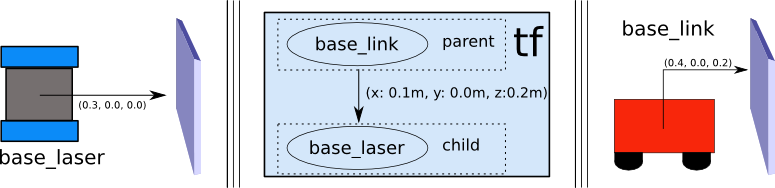
\includegraphics[width=0.5\textwidth,angle=0]{tutorials/tutorial_2/img/tf_robot.png}
		%\chapter*{Tutorial 3}

Create a new struct to send and receive from Server and Client.

\section{Client}
\begin{verbatim}

create a new file (process_X.cfg) for the configuration of the process

process(
	name = Process_X
	SHM = SHM_X
	Subscriber = cmd_vel
	Publisher = odom_1
 	Node2RTAI  = posWheels
	RTAI2Node  = posWheels
	IP_RTAI  = 140.78.133.43
	PORT_RTAI  = 1101
)

In the file "AaronMR_Robotic_Stack/Drivers/CB_TCP_RTAI/include/TCP_RTAI/comStruct.h" create a new struct:

  struct posWheels_t
  {
    Point pos_W[4];
  };


In the file "AaronMR_Robotic_Stack/Drivers/CB_TCP_RTAI/include/TCP_RTAI/structType_C.hpp", create a new subclass:

class struct_posWheels : public structType {

public:
    posWheels();
    int serialize(char* data2s);
    int Unserialize(char* data2us);
    void* set_Publisher(char* name);
    void* set_Subscriber(char* name);

    ros::NodeHandle n;
    ros::Publisher posWheels_pub;
    ros::Subscriber posWheels_sub;

    // struct to send and receive
    posWheels_t data2send;
    posWheels_t data2recv;

    geometry_msgs::Point point_msg;
    void cmdCallback(const geometry_msgs::Point &data_);
    bool haveSubscriber;
    bool havePublisher;
    pthread_mutex_t mutex;
    bool canRecv_t;
    bool canSend_t;
    bool canSend();
    bool canRecv();
    int spinOnce();
};


create a new file for the new class, "struct_posWheels.cpp" with the content:

#include "pack2.hpp"
#include "structType_C.hpp"

struct_posWheels::struct_posWheels()
{

}

void struct_posWheels::cmdCallback(const geometry_msgs::Point &data_)
{

}

void* struct_posWheels::set_Subscriber(char* name)
{

}

void* struct_posWheels::set_Publisher(char* name)
{

}

bool struct_posWheels::canSend()
{

}

bool struct_posWheels::canRecv()
{

}

int struct_posWheels::spinOnce()
{

}

int struct_posWheels::serialize(char* data2s)
{

}

int struct_posWheels::Unserialize(char* data2us)
{

}


In the constructor:

struct_posWheels::struct_posWheels()
{

    haveSubscriber  = false;
    havePublisher   = false;
    canRecv_t       = true;
    canSend_t       = true;
    mutex           = PTHREAD_MUTEX_INITIALIZER;

}


Configure the functions to serialize and unserialize:

int struct_posWheels::serialize(char* data2s)
{
   
    unsigned char buf[1024];
    unsigned char magic;
    unsigned int packetsize;
    unsigned int ps2;

    posWheels_t aux;

    aux.pos_W[0].x = 0.0;
    aux.pos_W[0].y = 0.0;
    aux.pos_W[0].z = 0.0;

    aux.pos_W[1].x = 0.0;
    aux.pos_W[1].y = 0.0;
    aux.pos_W[1].z = 0.0;

    aux.pos_W[2].x = 0.0;
    aux.pos_W[2].y = 0.0;
    aux.pos_W[2].z = 0.0;

    aux.pos_W[3].x = 0.0;
    aux.pos_W[3].y = 0.0;
    aux.pos_W[3].z = 0.0;

    packetsize = pack(buf, "CHdddddddddddd",  'A',
					      0,
                                              aux.pos_W[0].x,
                                              aux.pos_W[0].y,
                                              aux.pos_W[0].z,
                                              aux.pos_W[1].x,
                                              aux.pos_W[1].y,
                                              aux.pos_W[1].z,
                                              aux.pos_W[2].x,
                                              aux.pos_W[2].y,
                                              aux.pos_W[2].z,
                                              aux.pos_W[3].x,
                                              aux.pos_W[3].y,
                                              aux.pos_W[3].z);

    packi16(buf+1, packetsize); // store packet size in packet for kicks
    memcpy((unsigned char*)data2s, buf, packetsize);

    return 0;
}

int struct_posWheels::Unserialize(char* data2us)
{

    unsigned char buf[1024];
    unsigned char magic;
    unsigned int ps2;

    memcpy(buf, data2us, 1024);

    posWheels_t aux;

    aux.pos_W[0].x = 0.0;
    aux.pos_W[0].y = 0.0;
    aux.pos_W[0].z = 0.0;

    aux.pos_W[1].x = 0.0;
    aux.pos_W[1].y = 0.0;
    aux.pos_W[1].z = 0.0;

    aux.pos_W[2].x = 0.0;
    aux.pos_W[2].y = 0.0;
    aux.pos_W[2].z = 0.0;

    aux.pos_W[3].x = 0.0;
    aux.pos_W[3].y = 0.0;
    aux.pos_W[3].z = 0.0;

    unpack((unsigned char*)buf, "CHdddddddddddd",&magic,
                                                &ps2,
                                                &aux.pos_W[0].x,
                                                &aux.pos_W[0].y,
                                                &aux.pos_W[0].z,
                                                &aux.pos_W[1].x,
                                                &aux.pos_W[1].y,
                                                &aux.pos_W[1].z,
                                                &aux.pos_W[2].x,
                                                &aux.pos_W[2].y,
                                                &aux.pos_W[2].z,
                                                &aux.pos_W[3].x,
                                                &aux.pos_W[3].y,
                                                &aux.pos_W[3].z);


    return 0;
}


In the file "AaronMR_C.cpp", add the next lines:

// Configure type of struct to send
...
else if(configuration[0].Node2RTAI.compare("posWheels") == 0)
{
  structToSend = new struct_posWheels;
}

// configure type of struct to receive
...
else if(configuration[0].RTAI2Node.compare("posWheels") == 0)
{
  structToRecv = new struct_posWheels;
}

\end{verbatim}

\section{Server}

\begin{verbatim}

Add a new configuration in the file "ServerFile.cfg" for the configuration of the new process

process(
	name = Process_X
	SHM = SHM_X
	Subscriber = cmd_vel
	Publisher = odom_1
 	Node2RTAI  = posWheels
	RTAI2Node  = posWheels
	IP_RTAI  = 140.78.133.43
	PORT_RTAI  = 1101
)

In the file "comStruct.h" add the new struct_posWheels

struct posWheels_t
{
  Point pos_W[4];
}

Create a new class in the structType_S.cpp

    class struct_posWheels : public structType {
    public:
      struct_posWheels();
      char* serialize(char* data2s);
      char* Unserialize(char* data2us);
      void storeData(Joy *joy);
      Joy auxJoy1;

      void iniSHM(int shm_in, int shm_out, char* SHM_name);

      Pose auxPose1;
      int sizeof_Joy;
      bool haveSubscriber;
      bool havePublisher;

      struct posWheels_t *dataIN;
      struct posWheels_t *dataOUT;

    };

Create a new file for the new class, "struct_posWheels.cpp" with the content

#include "AaronMR_S.hpp"
#include "pack2.hpp"
#include <rtai_shm.h>

struct_posWheels::struct_posWheels()
{
   auxSerialize.pos_W[0].x = 0.0;
   auxSerialize.pos_W[0].y = 0.0;
   auxSerialize.pos_W[0].z = 0.0;

   auxSerialize.pos_W[1].x = 0.0;
   auxSerialize.pos_W[1].y = 0.0;
   auxSerialize.pos_W[1].z = 0.0;

   auxSerialize.pos_W[2].x = 0.0;
   auxSerialize.pos_W[2].y = 0.0;
   auxSerialize.pos_W[2].z = 0.0;

   auxSerialize.pos_W[3].x = 0.0;
   auxSerialize.pos_W[3].y = 0.0;
   auxSerialize.pos_W[3].z = 0.0;

   auxUnSerialize.pos_W[0].x = 0.0;
   auxUnSerialize.pos_W[0].y = 0.0;
   auxUnSerialize.pos_W[0].z = 0.0;

   auxUnSerialize.pos_W[1].x = 0.0;
   auxUnSerialize.pos_W[1].y = 0.0;
   auxUnSerialize.pos_W[1].z = 0.0;

   auxUnSerialize.pos_W[2].x = 0.0;
   auxUnSerialize.pos_W[2].y = 0.0;
   auxUnSerialize.pos_W[2].z = 0.0;

   auxUnSerialize.pos_W[3].x = 0.0;
   auxUnSerialize.pos_W[3].y = 0.0;
   auxUnSerialize.pos_W[3].z = 0.0;

}

void struct_posWheels::iniSHM(int shm_in, int shm_out, char* SHM_name)
{
   if (shm_in == 1)
   {
       dataIN = (posWheels_t*)rtai_malloc (nam2num(SHM_name), sizeof(struct posWheels_t)) ;

       dataIN->pos_W[0].x = 0.1;
       dataIN->pos_W[0].y = 0.2;
       dataIN->pos_W[0].z = 0.3;

       dataIN->pos_W[1].x = 0.4;
       dataIN->pos_W[1].y = 0.5;
       dataIN->pos_W[1].z = 0.6;

       dataIN->pos_W[2].x = 0.7;
       dataIN->pos_W[2].y = 0.8;
       dataIN->pos_W[2].z = 0.9;

       dataIN->pos_W[3].x = 0.10;
       dataIN->pos_W[3].y = 0.11;
       dataIN->pos_W[3].z = 0.12;
   }

   if (shm_out == 1)
   {
       dataOUT = (posWheels_t*)rtai_malloc (nam2num(SHM_name), sizeof(struct posWheels_t)) ;

       dataOUT->pos_W[0].x = 1.0;
       dataOUT->pos_W[0].y = 2.0;
       dataOUT->pos_W[0].z = 3.0;

       dataOUT->pos_W[1].x = 4.0;
       dataOUT->pos_W[1].y = 5.0;
       dataOUT->pos_W[1].z = 6.0;

       dataOUT->pos_W[2].x = 7.0;
       dataOUT->pos_W[2].y = 8.0;
       dataOUT->pos_W[2].z = 9.0;

       dataOUT->pos_W[3].x = 10.0;
       dataOUT->pos_W[3].y = 11.0;
       dataOUT->pos_W[3].z = 12.0;
   }
}

char *struct_posWheels::serialize(char* buf3)
{
    unsigned char buf[1024];
    unsigned char magic;
    unsigned int packetsize, ps2;

   auxSerialize.pos_W[0].x = dataOUT->pos_W[0].x;
   auxSerialize.pos_W[0].y = dataOUT->pos_W[0].y;
   auxSerialize.pos_W[0].z = dataOUT->pos_W[0].z;

   auxSerialize.pos_W[1].x = dataOUT->pos_W[1].x;
   auxSerialize.pos_W[1].y = dataOUT->pos_W[1].y;
   auxSerialize.pos_W[1].z = dataOUT->pos_W[1].z;

   auxSerialize.pos_W[2].x = dataOUT->pos_W[2].x;
   auxSerialize.pos_W[2].y = dataOUT->pos_W[2].y;
   auxSerialize.pos_W[2].z = dataOUT->pos_W[2].z;

   auxSerialize.pos_W[3].x = dataOUT->pos_W[3].x;
   auxSerialize.pos_W[3].y = dataOUT->pos_W[3].y;
   auxSerialize.pos_W[3].z = dataOUT->pos_W[3].z;

   packetsize = pack(buf, "CHdddddddddddd", 'A',
                                       0,
                                       auxSerialize.pos_W[0].x,
                                       auxSerialize.pos_W[0].y,
                                       auxSerialize.pos_W[0].z,
                                       auxSerialize.pos_W[1].x,
                                       auxSerialize.pos_W[1].y,
                                       auxSerialize.pos_W[1].z,
                                       auxSerialize.pos_W[2].x,
                                       auxSerialize.pos_W[2].y,
                                       auxSerialize.pos_W[2].z,
                                       auxSerialize.pos_W[3].x,
                                       auxSerialize.pos_W[3].y,
                                       auxSerialize.pos_W[3].z
                                       );

   packi16(buf+1, packetsize); // store packet size in packet for kicks

   memcpy((unsigned char*)buf3, buf, packetsize);

    unpack((unsigned char*)buf3, "CHdddddddddddd",
                                           &magic,
                                           &ps2,
                                           &auxSerialize.pos_W[0].x,
                                           &auxSerialize.pos_W[0].y,
                                           &auxSerialize.pos_W[0].z,
                                           &auxSerialize.pos_W[1].x,
                                           &auxSerialize.pos_W[1].y,
                                           &auxSerialize.pos_W[1].z,
                                           &auxSerialize.pos_W[2].x,
                                           &auxSerialize.pos_W[2].y,
                                           &auxSerialize.pos_W[2].z,
                                           &auxSerialize.pos_W[3].x,
                                           &auxSerialize.pos_W[3].y,
                                           &auxSerialize.pos_W[3].z
                                           );

    printf("posWheels - send: '%c' %hhu %f %f %f %f %f %f %f %f %f %f %f %f\n",
                                           magic,
                                           ps2,
                                           auxSerialize.pos_W[0].x,
                                           auxSerialize.pos_W[0].y,
                                           auxSerialize.pos_W[0].z,
                                           auxSerialize.pos_W[1].x,
                                           auxSerialize.pos_W[1].y,
                                           auxSerialize.pos_W[1].z,
                                           auxSerialize.pos_W[2].x,
                                           auxSerialize.pos_W[2].y,
                                           auxSerialize.pos_W[2].z,
                                           auxSerialize.pos_W[3].x,
                                           auxSerialize.pos_W[3].y,
                                           auxSerialize.pos_W[3].z
                                           );

}

char *struct_posWheels::Unserialize(char* buf3)
{

   unsigned char buf[1024];
    unsigned char magic;
    unsigned int ps2;

   memcpy(buf, buf3, 1024);

    unpack((unsigned char*)buf, "CHdddddddddddd",
                                           &magic,
                                           &ps2,
                                           &auxUnSerialize.pos_W[0].x,
                                           &auxUnSerialize.pos_W[0].y,
                                           &auxUnSerialize.pos_W[0].z,
                                           &auxUnSerialize.pos_W[1].x,
                                           &auxUnSerialize.pos_W[1].y,
                                           &auxUnSerialize.pos_W[1].z,
                                           &auxUnSerialize.pos_W[2].x,
                                           &auxUnSerialize.pos_W[2].y,
                                           &auxUnSerialize.pos_W[2].z,
                                           &auxUnSerialize.pos_W[3].x,
                                           &auxUnSerialize.pos_W[3].y,
                                           &auxUnSerialize.pos_W[3].z
                                           );

    printf("posWheels - recv: '%c' %hhu %f %f %f %f %f %f %f %f %f %f %f %f\n",
                                           magic,
                                           ps2,
                                           auxUnSerialize.pos_W[0].x,
                                           auxUnSerialize.pos_W[0].y,
                                           auxUnSerialize.pos_W[0].z,
                                           auxUnSerialize.pos_W[1].x,
                                           auxUnSerialize.pos_W[1].y,
                                           auxUnSerialize.pos_W[1].z,
                                           auxUnSerialize.pos_W[2].x,
                                           auxUnSerialize.pos_W[2].y,
                                           auxUnSerialize.pos_W[2].z,
                                           auxUnSerialize.pos_W[3].x,
                                           auxUnSerialize.pos_W[3].y,
                                           auxUnSerialize.pos_W[3].z
                                           );

   dataIN->pos_W[0].x = auxUnSerialize.pos_W[0].x;
   dataIN->pos_W[0].y = auxUnSerialize.pos_W[0].y;
   dataIN->pos_W[0].z = auxUnSerialize.pos_W[0].z;

   dataIN->pos_W[1].x = auxUnSerialize.pos_W[1].x;
   dataIN->pos_W[1].y = auxUnSerialize.pos_W[1].y;
   dataIN->pos_W[1].z = auxUnSerialize.pos_W[1].z;

   dataIN->pos_W[2].x = auxUnSerialize.pos_W[2].x;
   dataIN->pos_W[2].y = auxUnSerialize.pos_W[2].y;
   dataIN->pos_W[2].z = auxUnSerialize.pos_W[2].z;

   dataIN->pos_W[3].x = auxUnSerialize.pos_W[3].x;
   dataIN->pos_W[3].y = auxUnSerialize.pos_W[3].y;
   dataIN->pos_W[3].z = auxUnSerialize.pos_W[3].z;

   return NULL;
}


Add the next lines in the "AaronMR_S.cpp" file

// configuration send structure
  ...
  ...
}else if(processThread_2.Node2RTAI.compare("posWheels") == 0){
       //Node2RTAI = 6;
       structToRecv = new struct_posWheels;
       structToRecv->iniSHM(1, 0, (char*)processThread_2.SHM_IN.data());
}

...
...
// configuration recv structure
  ...
  ...
}else if(processThread_2.RTAI2Node.compare("posWheels") == 0){
       //RTAI2Node = 6;
       structToSend = new struct_posWheels;
       structToSend->iniSHM(0,1, (char*)processThread_2.SHM_OUT.data());
}

\end{verbatim}


%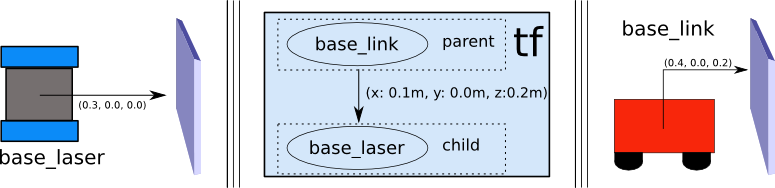
\includegraphics[width=0.5\textwidth,angle=0]{tutorials/tutorial_2/img/tf_robot.png}
		%\include{Navigation}
		%\chapter*{Tutorial 3}

Create a new struct to send and receive from Server and Client.

\section{Client}
\begin{verbatim}

create a new file (process_X.cfg) for the configuration of the process

process(
	name = Process_X
	SHM = SHM_X
	Subscriber = cmd_vel
	Publisher = odom_1
 	Node2RTAI  = posWheels
	RTAI2Node  = posWheels
	IP_RTAI  = 140.78.133.43
	PORT_RTAI  = 1101
)

In the file "AaronMR_Robotic_Stack/Drivers/CB_TCP_RTAI/include/TCP_RTAI/comStruct.h" create a new struct:

  struct posWheels_t
  {
    Point pos_W[4];
  };


In the file "AaronMR_Robotic_Stack/Drivers/CB_TCP_RTAI/include/TCP_RTAI/structType_C.hpp", create a new subclass:

class struct_posWheels : public structType {

public:
    posWheels();
    int serialize(char* data2s);
    int Unserialize(char* data2us);
    void* set_Publisher(char* name);
    void* set_Subscriber(char* name);

    ros::NodeHandle n;
    ros::Publisher posWheels_pub;
    ros::Subscriber posWheels_sub;

    // struct to send and receive
    posWheels_t data2send;
    posWheels_t data2recv;

    geometry_msgs::Point point_msg;
    void cmdCallback(const geometry_msgs::Point &data_);
    bool haveSubscriber;
    bool havePublisher;
    pthread_mutex_t mutex;
    bool canRecv_t;
    bool canSend_t;
    bool canSend();
    bool canRecv();
    int spinOnce();
};


create a new file for the new class, "struct_posWheels.cpp" with the content:

#include "pack2.hpp"
#include "structType_C.hpp"

struct_posWheels::struct_posWheels()
{

}

void struct_posWheels::cmdCallback(const geometry_msgs::Point &data_)
{

}

void* struct_posWheels::set_Subscriber(char* name)
{

}

void* struct_posWheels::set_Publisher(char* name)
{

}

bool struct_posWheels::canSend()
{

}

bool struct_posWheels::canRecv()
{

}

int struct_posWheels::spinOnce()
{

}

int struct_posWheels::serialize(char* data2s)
{

}

int struct_posWheels::Unserialize(char* data2us)
{

}


In the constructor:

struct_posWheels::struct_posWheels()
{

    haveSubscriber  = false;
    havePublisher   = false;
    canRecv_t       = true;
    canSend_t       = true;
    mutex           = PTHREAD_MUTEX_INITIALIZER;

}


Configure the functions to serialize and unserialize:

int struct_posWheels::serialize(char* data2s)
{
   
    unsigned char buf[1024];
    unsigned char magic;
    unsigned int packetsize;
    unsigned int ps2;

    posWheels_t aux;

    aux.pos_W[0].x = 0.0;
    aux.pos_W[0].y = 0.0;
    aux.pos_W[0].z = 0.0;

    aux.pos_W[1].x = 0.0;
    aux.pos_W[1].y = 0.0;
    aux.pos_W[1].z = 0.0;

    aux.pos_W[2].x = 0.0;
    aux.pos_W[2].y = 0.0;
    aux.pos_W[2].z = 0.0;

    aux.pos_W[3].x = 0.0;
    aux.pos_W[3].y = 0.0;
    aux.pos_W[3].z = 0.0;

    packetsize = pack(buf, "CHdddddddddddd",  'A',
					      0,
                                              aux.pos_W[0].x,
                                              aux.pos_W[0].y,
                                              aux.pos_W[0].z,
                                              aux.pos_W[1].x,
                                              aux.pos_W[1].y,
                                              aux.pos_W[1].z,
                                              aux.pos_W[2].x,
                                              aux.pos_W[2].y,
                                              aux.pos_W[2].z,
                                              aux.pos_W[3].x,
                                              aux.pos_W[3].y,
                                              aux.pos_W[3].z);

    packi16(buf+1, packetsize); // store packet size in packet for kicks
    memcpy((unsigned char*)data2s, buf, packetsize);

    return 0;
}

int struct_posWheels::Unserialize(char* data2us)
{

    unsigned char buf[1024];
    unsigned char magic;
    unsigned int ps2;

    memcpy(buf, data2us, 1024);

    posWheels_t aux;

    aux.pos_W[0].x = 0.0;
    aux.pos_W[0].y = 0.0;
    aux.pos_W[0].z = 0.0;

    aux.pos_W[1].x = 0.0;
    aux.pos_W[1].y = 0.0;
    aux.pos_W[1].z = 0.0;

    aux.pos_W[2].x = 0.0;
    aux.pos_W[2].y = 0.0;
    aux.pos_W[2].z = 0.0;

    aux.pos_W[3].x = 0.0;
    aux.pos_W[3].y = 0.0;
    aux.pos_W[3].z = 0.0;

    unpack((unsigned char*)buf, "CHdddddddddddd",&magic,
                                                &ps2,
                                                &aux.pos_W[0].x,
                                                &aux.pos_W[0].y,
                                                &aux.pos_W[0].z,
                                                &aux.pos_W[1].x,
                                                &aux.pos_W[1].y,
                                                &aux.pos_W[1].z,
                                                &aux.pos_W[2].x,
                                                &aux.pos_W[2].y,
                                                &aux.pos_W[2].z,
                                                &aux.pos_W[3].x,
                                                &aux.pos_W[3].y,
                                                &aux.pos_W[3].z);


    return 0;
}


In the file "AaronMR_C.cpp", add the next lines:

// Configure type of struct to send
...
else if(configuration[0].Node2RTAI.compare("posWheels") == 0)
{
  structToSend = new struct_posWheels;
}

// configure type of struct to receive
...
else if(configuration[0].RTAI2Node.compare("posWheels") == 0)
{
  structToRecv = new struct_posWheels;
}

\end{verbatim}

\section{Server}

\begin{verbatim}

Add a new configuration in the file "ServerFile.cfg" for the configuration of the new process

process(
	name = Process_X
	SHM = SHM_X
	Subscriber = cmd_vel
	Publisher = odom_1
 	Node2RTAI  = posWheels
	RTAI2Node  = posWheels
	IP_RTAI  = 140.78.133.43
	PORT_RTAI  = 1101
)

In the file "comStruct.h" add the new struct_posWheels

struct posWheels_t
{
  Point pos_W[4];
}

Create a new class in the structType_S.cpp

    class struct_posWheels : public structType {
    public:
      struct_posWheels();
      char* serialize(char* data2s);
      char* Unserialize(char* data2us);
      void storeData(Joy *joy);
      Joy auxJoy1;

      void iniSHM(int shm_in, int shm_out, char* SHM_name);

      Pose auxPose1;
      int sizeof_Joy;
      bool haveSubscriber;
      bool havePublisher;

      struct posWheels_t *dataIN;
      struct posWheels_t *dataOUT;

    };

Create a new file for the new class, "struct_posWheels.cpp" with the content

#include "AaronMR_S.hpp"
#include "pack2.hpp"
#include <rtai_shm.h>

struct_posWheels::struct_posWheels()
{
   auxSerialize.pos_W[0].x = 0.0;
   auxSerialize.pos_W[0].y = 0.0;
   auxSerialize.pos_W[0].z = 0.0;

   auxSerialize.pos_W[1].x = 0.0;
   auxSerialize.pos_W[1].y = 0.0;
   auxSerialize.pos_W[1].z = 0.0;

   auxSerialize.pos_W[2].x = 0.0;
   auxSerialize.pos_W[2].y = 0.0;
   auxSerialize.pos_W[2].z = 0.0;

   auxSerialize.pos_W[3].x = 0.0;
   auxSerialize.pos_W[3].y = 0.0;
   auxSerialize.pos_W[3].z = 0.0;

   auxUnSerialize.pos_W[0].x = 0.0;
   auxUnSerialize.pos_W[0].y = 0.0;
   auxUnSerialize.pos_W[0].z = 0.0;

   auxUnSerialize.pos_W[1].x = 0.0;
   auxUnSerialize.pos_W[1].y = 0.0;
   auxUnSerialize.pos_W[1].z = 0.0;

   auxUnSerialize.pos_W[2].x = 0.0;
   auxUnSerialize.pos_W[2].y = 0.0;
   auxUnSerialize.pos_W[2].z = 0.0;

   auxUnSerialize.pos_W[3].x = 0.0;
   auxUnSerialize.pos_W[3].y = 0.0;
   auxUnSerialize.pos_W[3].z = 0.0;

}

void struct_posWheels::iniSHM(int shm_in, int shm_out, char* SHM_name)
{
   if (shm_in == 1)
   {
       dataIN = (posWheels_t*)rtai_malloc (nam2num(SHM_name), sizeof(struct posWheels_t)) ;

       dataIN->pos_W[0].x = 0.1;
       dataIN->pos_W[0].y = 0.2;
       dataIN->pos_W[0].z = 0.3;

       dataIN->pos_W[1].x = 0.4;
       dataIN->pos_W[1].y = 0.5;
       dataIN->pos_W[1].z = 0.6;

       dataIN->pos_W[2].x = 0.7;
       dataIN->pos_W[2].y = 0.8;
       dataIN->pos_W[2].z = 0.9;

       dataIN->pos_W[3].x = 0.10;
       dataIN->pos_W[3].y = 0.11;
       dataIN->pos_W[3].z = 0.12;
   }

   if (shm_out == 1)
   {
       dataOUT = (posWheels_t*)rtai_malloc (nam2num(SHM_name), sizeof(struct posWheels_t)) ;

       dataOUT->pos_W[0].x = 1.0;
       dataOUT->pos_W[0].y = 2.0;
       dataOUT->pos_W[0].z = 3.0;

       dataOUT->pos_W[1].x = 4.0;
       dataOUT->pos_W[1].y = 5.0;
       dataOUT->pos_W[1].z = 6.0;

       dataOUT->pos_W[2].x = 7.0;
       dataOUT->pos_W[2].y = 8.0;
       dataOUT->pos_W[2].z = 9.0;

       dataOUT->pos_W[3].x = 10.0;
       dataOUT->pos_W[3].y = 11.0;
       dataOUT->pos_W[3].z = 12.0;
   }
}

char *struct_posWheels::serialize(char* buf3)
{
    unsigned char buf[1024];
    unsigned char magic;
    unsigned int packetsize, ps2;

   auxSerialize.pos_W[0].x = dataOUT->pos_W[0].x;
   auxSerialize.pos_W[0].y = dataOUT->pos_W[0].y;
   auxSerialize.pos_W[0].z = dataOUT->pos_W[0].z;

   auxSerialize.pos_W[1].x = dataOUT->pos_W[1].x;
   auxSerialize.pos_W[1].y = dataOUT->pos_W[1].y;
   auxSerialize.pos_W[1].z = dataOUT->pos_W[1].z;

   auxSerialize.pos_W[2].x = dataOUT->pos_W[2].x;
   auxSerialize.pos_W[2].y = dataOUT->pos_W[2].y;
   auxSerialize.pos_W[2].z = dataOUT->pos_W[2].z;

   auxSerialize.pos_W[3].x = dataOUT->pos_W[3].x;
   auxSerialize.pos_W[3].y = dataOUT->pos_W[3].y;
   auxSerialize.pos_W[3].z = dataOUT->pos_W[3].z;

   packetsize = pack(buf, "CHdddddddddddd", 'A',
                                       0,
                                       auxSerialize.pos_W[0].x,
                                       auxSerialize.pos_W[0].y,
                                       auxSerialize.pos_W[0].z,
                                       auxSerialize.pos_W[1].x,
                                       auxSerialize.pos_W[1].y,
                                       auxSerialize.pos_W[1].z,
                                       auxSerialize.pos_W[2].x,
                                       auxSerialize.pos_W[2].y,
                                       auxSerialize.pos_W[2].z,
                                       auxSerialize.pos_W[3].x,
                                       auxSerialize.pos_W[3].y,
                                       auxSerialize.pos_W[3].z
                                       );

   packi16(buf+1, packetsize); // store packet size in packet for kicks

   memcpy((unsigned char*)buf3, buf, packetsize);

    unpack((unsigned char*)buf3, "CHdddddddddddd",
                                           &magic,
                                           &ps2,
                                           &auxSerialize.pos_W[0].x,
                                           &auxSerialize.pos_W[0].y,
                                           &auxSerialize.pos_W[0].z,
                                           &auxSerialize.pos_W[1].x,
                                           &auxSerialize.pos_W[1].y,
                                           &auxSerialize.pos_W[1].z,
                                           &auxSerialize.pos_W[2].x,
                                           &auxSerialize.pos_W[2].y,
                                           &auxSerialize.pos_W[2].z,
                                           &auxSerialize.pos_W[3].x,
                                           &auxSerialize.pos_W[3].y,
                                           &auxSerialize.pos_W[3].z
                                           );

    printf("posWheels - send: '%c' %hhu %f %f %f %f %f %f %f %f %f %f %f %f\n",
                                           magic,
                                           ps2,
                                           auxSerialize.pos_W[0].x,
                                           auxSerialize.pos_W[0].y,
                                           auxSerialize.pos_W[0].z,
                                           auxSerialize.pos_W[1].x,
                                           auxSerialize.pos_W[1].y,
                                           auxSerialize.pos_W[1].z,
                                           auxSerialize.pos_W[2].x,
                                           auxSerialize.pos_W[2].y,
                                           auxSerialize.pos_W[2].z,
                                           auxSerialize.pos_W[3].x,
                                           auxSerialize.pos_W[3].y,
                                           auxSerialize.pos_W[3].z
                                           );

}

char *struct_posWheels::Unserialize(char* buf3)
{

   unsigned char buf[1024];
    unsigned char magic;
    unsigned int ps2;

   memcpy(buf, buf3, 1024);

    unpack((unsigned char*)buf, "CHdddddddddddd",
                                           &magic,
                                           &ps2,
                                           &auxUnSerialize.pos_W[0].x,
                                           &auxUnSerialize.pos_W[0].y,
                                           &auxUnSerialize.pos_W[0].z,
                                           &auxUnSerialize.pos_W[1].x,
                                           &auxUnSerialize.pos_W[1].y,
                                           &auxUnSerialize.pos_W[1].z,
                                           &auxUnSerialize.pos_W[2].x,
                                           &auxUnSerialize.pos_W[2].y,
                                           &auxUnSerialize.pos_W[2].z,
                                           &auxUnSerialize.pos_W[3].x,
                                           &auxUnSerialize.pos_W[3].y,
                                           &auxUnSerialize.pos_W[3].z
                                           );

    printf("posWheels - recv: '%c' %hhu %f %f %f %f %f %f %f %f %f %f %f %f\n",
                                           magic,
                                           ps2,
                                           auxUnSerialize.pos_W[0].x,
                                           auxUnSerialize.pos_W[0].y,
                                           auxUnSerialize.pos_W[0].z,
                                           auxUnSerialize.pos_W[1].x,
                                           auxUnSerialize.pos_W[1].y,
                                           auxUnSerialize.pos_W[1].z,
                                           auxUnSerialize.pos_W[2].x,
                                           auxUnSerialize.pos_W[2].y,
                                           auxUnSerialize.pos_W[2].z,
                                           auxUnSerialize.pos_W[3].x,
                                           auxUnSerialize.pos_W[3].y,
                                           auxUnSerialize.pos_W[3].z
                                           );

   dataIN->pos_W[0].x = auxUnSerialize.pos_W[0].x;
   dataIN->pos_W[0].y = auxUnSerialize.pos_W[0].y;
   dataIN->pos_W[0].z = auxUnSerialize.pos_W[0].z;

   dataIN->pos_W[1].x = auxUnSerialize.pos_W[1].x;
   dataIN->pos_W[1].y = auxUnSerialize.pos_W[1].y;
   dataIN->pos_W[1].z = auxUnSerialize.pos_W[1].z;

   dataIN->pos_W[2].x = auxUnSerialize.pos_W[2].x;
   dataIN->pos_W[2].y = auxUnSerialize.pos_W[2].y;
   dataIN->pos_W[2].z = auxUnSerialize.pos_W[2].z;

   dataIN->pos_W[3].x = auxUnSerialize.pos_W[3].x;
   dataIN->pos_W[3].y = auxUnSerialize.pos_W[3].y;
   dataIN->pos_W[3].z = auxUnSerialize.pos_W[3].z;

   return NULL;
}


Add the next lines in the "AaronMR_S.cpp" file

// configuration send structure
  ...
  ...
}else if(processThread_2.Node2RTAI.compare("posWheels") == 0){
       //Node2RTAI = 6;
       structToRecv = new struct_posWheels;
       structToRecv->iniSHM(1, 0, (char*)processThread_2.SHM_IN.data());
}

...
...
// configuration recv structure
  ...
  ...
}else if(processThread_2.RTAI2Node.compare("posWheels") == 0){
       //RTAI2Node = 6;
       structToSend = new struct_posWheels;
       structToSend->iniSHM(0,1, (char*)processThread_2.SHM_OUT.data());
}

\end{verbatim}


%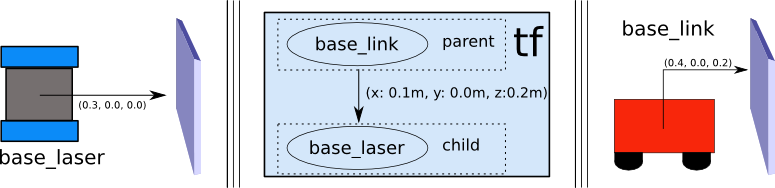
\includegraphics[width=0.5\textwidth,angle=0]{tutorials/tutorial_2/img/tf_robot.png}


\end{document}
